\chapter{Project Evolution}
\label{chap:projectevolution}
\section{Initial Idea}
\label{sec:projectevolution_initialproblem}

The original plan for this project was to create an asset for the Unity Asset Store that would provide a generic interface for implementing computer controlled units, primarily for tour guides. It would have various aspects that a tour guide would need to function, such as a waypoint system, text-to-speech, path finding and other features. The same tool could also be used to program other bots, such as a zombie or a villager in video games, as they require similar behaviour.

\begin{figure}[H]
	\centering
		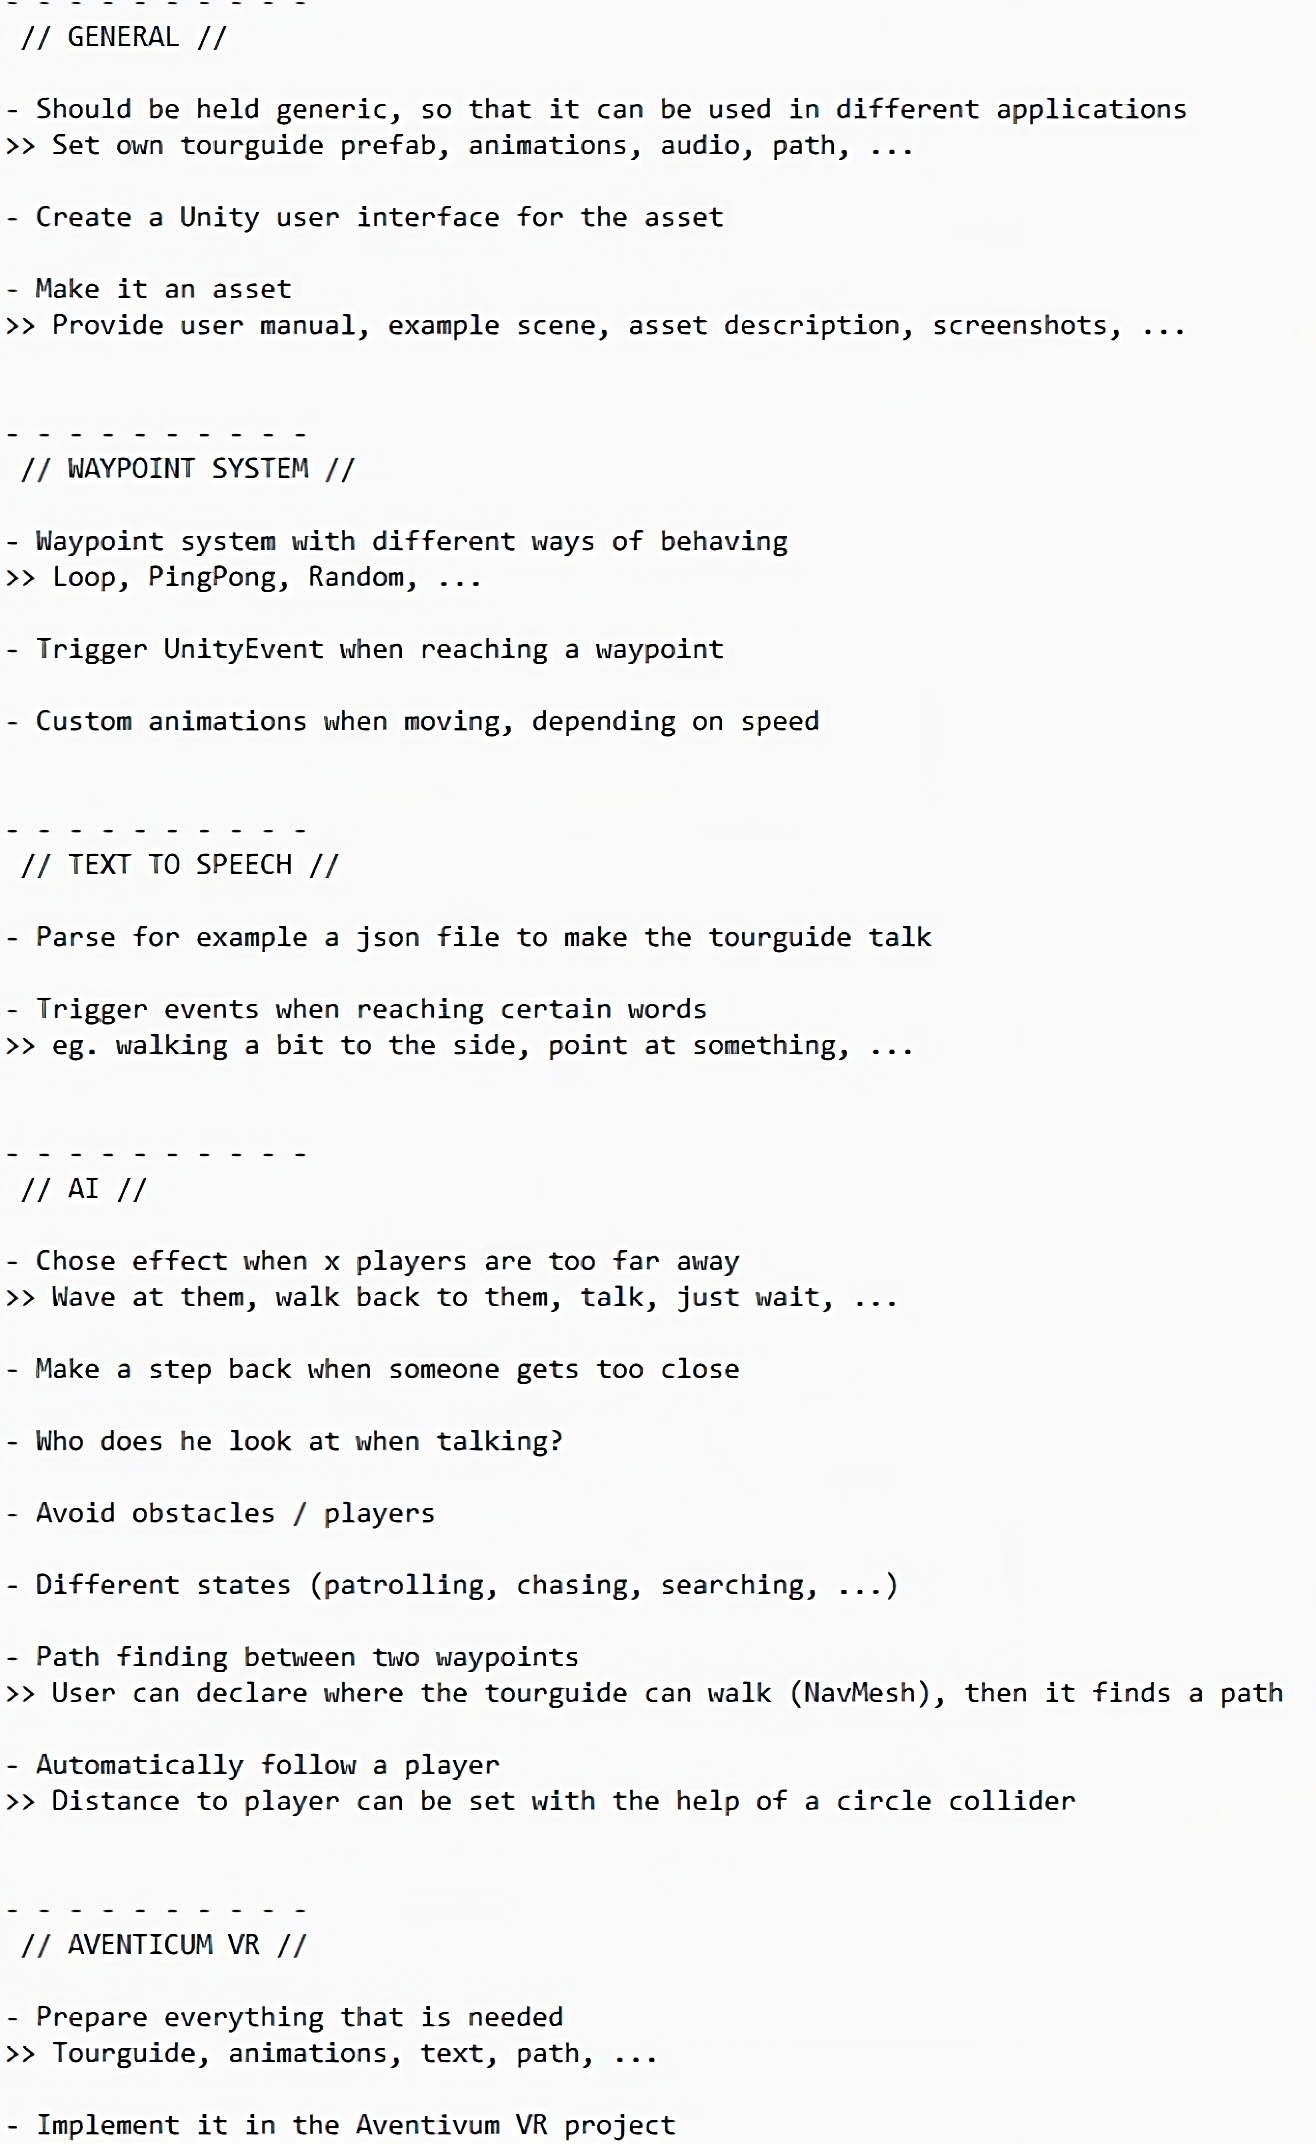
\includegraphics[scale=0.205]{images/bot_controller_idea.png}
	\caption{First Ideas}
	\label{fig:bot_controller_idea}
\end{figure}

Figure \ref{fig:bot_controller_idea} shows the parts into which the project was divided. In the Unity editor, the user could add this asset as a component to the unit they wanted this tool to control. This component could then be edited in the inspector window. The options available for configuring it would be as shown in the figure \ref{fig:bot_controller_idea}. To achieve this goal, the component would have to be created using the Unity editor scripting by deriving from the Editor class. This class provides all the functionality needed to customise the functionality and appearance of the inspector.

\begin{figure}[H]
	\centering
		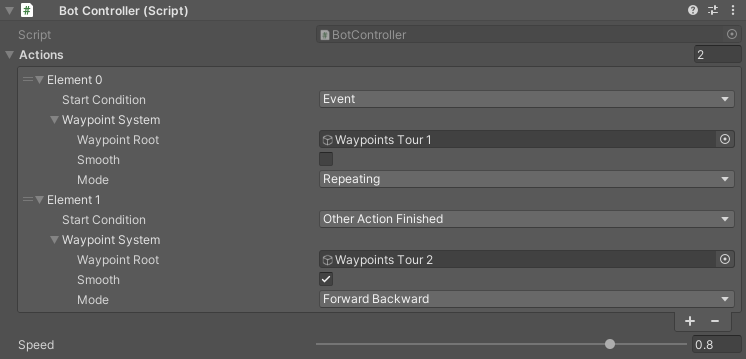
\includegraphics[scale=0.6]{images/bot_controller_gui.png}
	\caption{Example of the GUI in Unity}
	\label{fig:bot_controller_gui}
\end{figure}

This is an example of what an interface created with the Editor class might look like. It's a good visualisation of what part of this tool might look like when it's finished. A new action can be created by clicking on the "+" icon at the bottom right. How exactly the action is triggered can be selected from the "Start Condition" drop down. Once executed, the action would cause the GameObject to which the script is attached to follow the specified waypoints assigned in the "Waypoint Root" field. Once the whole asset was finished, it would have more functionality than just a waypoint system, and would therefore become much more complex.

\begin{figure}[H]
  \centering
  \begin{minipage}{0.45\textwidth}
    \centering
    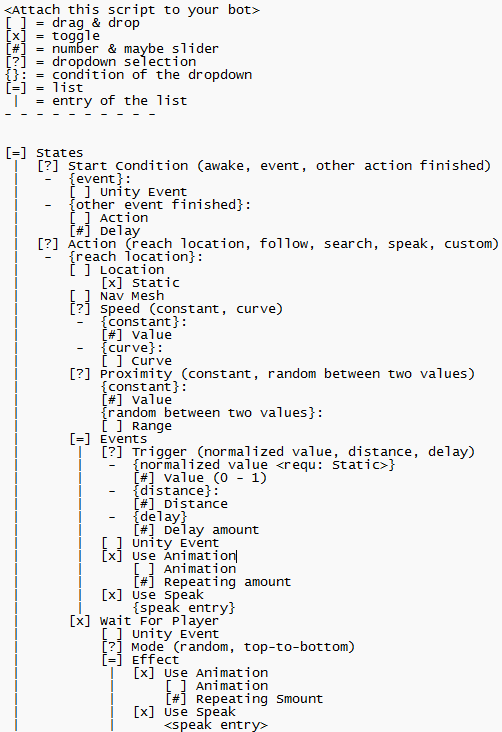
\includegraphics[scale=0.55]{images/bot_contoller_features_1.png}
    \caption{Features page 1}
    \label{fig:bot_contoller_features_1}
  \end{minipage}
  \hfill
  \begin{minipage}{0.45\textwidth}
    \centering
    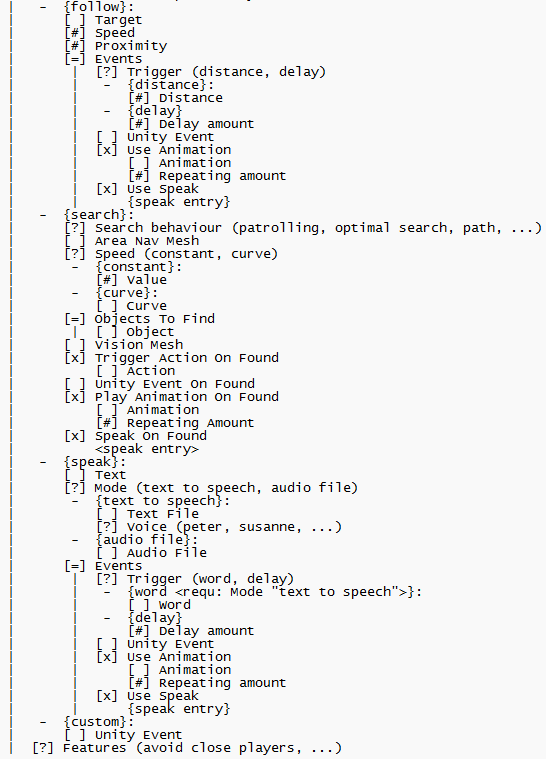
\includegraphics[scale=0.55]{images/bot_contoller_features_2.png}
    \caption{Features page 2}
    \label{fig:bot_contoller_features_2}
  \end{minipage}
  \caption{Features}
  \label{fig:bot_contoller_features}
\end{figure}

This is a sketch of what it might look like with all the features planned so far. At the top is a legend explaining what the symbols mean, and below is a hierarchical structure that allows the user to change the behaviour of this component.

It's a bit hard to understand at first, so here's an explanation of how it works:

The whole system works as a state machine, and new states could be added at will. Each state could be associated with a particular type of action, in the example of figure \ref{fig:bot_contoller_features}, the choices would be "reach location", "follow", "search", "speak" or a custom one. Each of these actions could have different variables to customise its behaviour. A "Start Condition" could be selected to define when an action should start. During an action, events could be triggered which could be used by the programmer or alternatively cause a change of state.

With this approach, the developer would have the option of either selecting one of the predefined actions or creating a new one. This could be used to create a behaviour in a relatively short amount of time.

\newpage

\section{Trouble}
\label{sec:projectevolution_trouble}

The problem with this solution is that the whole structure becomes very messy and hard to read as the number of actions grows. The main reason for this is that it becomes hard to see which state leads to which, and because it's a state machine, the number of states and links between them can grow quite quickly. So a graphical approach might help against this problem. If each action were a node in a graph, it would be much easier to see how everything is connected.

\section{Better Approach}
\label{sec:projectevolution_betterapproach}

The next idea was to implement this generic behaviour creator as a sequence graph. Each node represents an action, and each of these nodes can be freely connected to other nodes by an edge. In order for a state change to occur, a particular event must occur on the currently executing node.

\begin{figure}[H]
	\centering
		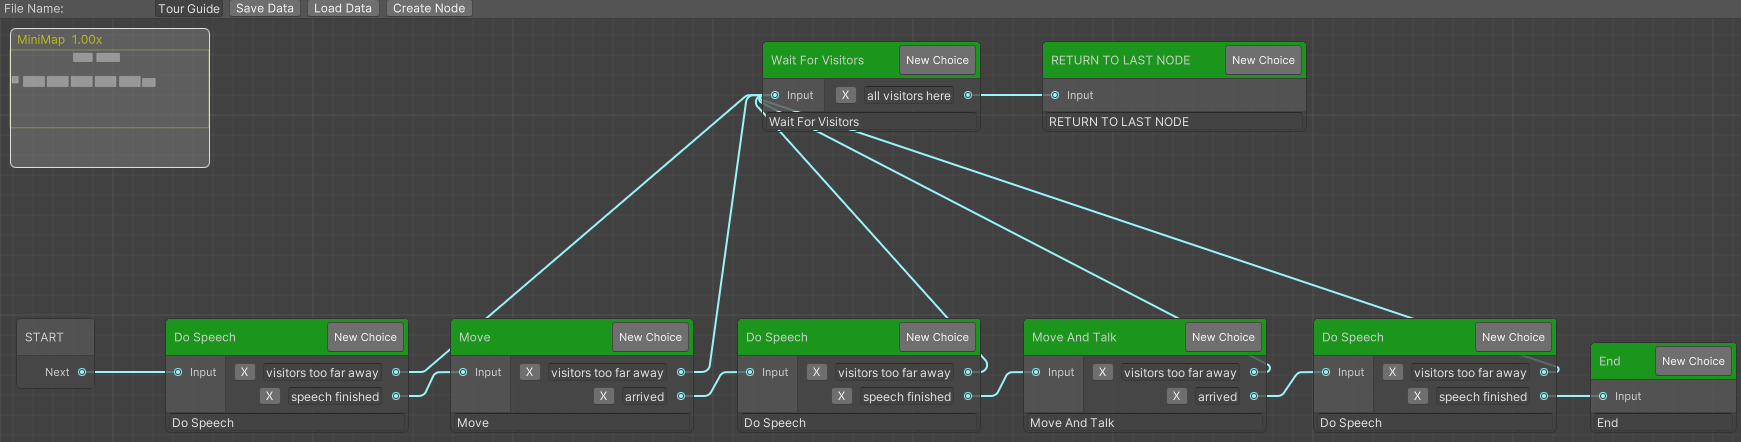
\includegraphics[scale=0.34]{images/sequence_graph_tour_guide.png}
	\caption{Sequence graph example for tour guide}
	\label{fig:sequence_graph_tour_guide}
\end{figure}

This graphic shows a very simple version of what a tour guide system might look like when it's finished. It was implemented to get more familiar with how programming a graphical interface for Unity works, and also to find out its advantages compared to scripting in the editor. Each node represents an action that the agent can perform, and each edge leads to a state change that can be triggered by one of the conditions.


For example, in figure \ref{fig:sequence_graph_tour_guide}, the behaviour would start at the "START" node on the left. It would immediately start executing the first "Do Speech" action, looking for triggers that a visitor is too far away or that the speech is finished. If one of the conditions for a trigger is met, a state change will take place. In the example of a visitor being too far away, the tour guide would go to the node at the top and perform the action "Wait for Visitors". As soon as the visitors are close enough again, the tour guide would continue his speech until the visitors are too far away again or the speech is finished. This behaviour will continue until the "End" node is reached, at which point it will stop.

By using a sequence graph, the whole structure looks more organised and nodes can be freely moved around and connected to other nodes. This makes it easier for the user to create the right behaviour for their application. The conditions for triggering the next action can also be programmed separately, allowing the same trigger to be used in multiple nodes, reducing the amount of scripting required.

\section{Why It Fails}
\label{sec:projectevolution_whyitfails}

Essentially, the whole structure is just a finite state machine (FSM), optimised mainly for implementing a tour guide. There are several problems with such an approach. One is that once there are many edges, it becomes difficult to understand which edge leads to which state.

\begin{figure}[H]
	\centering
		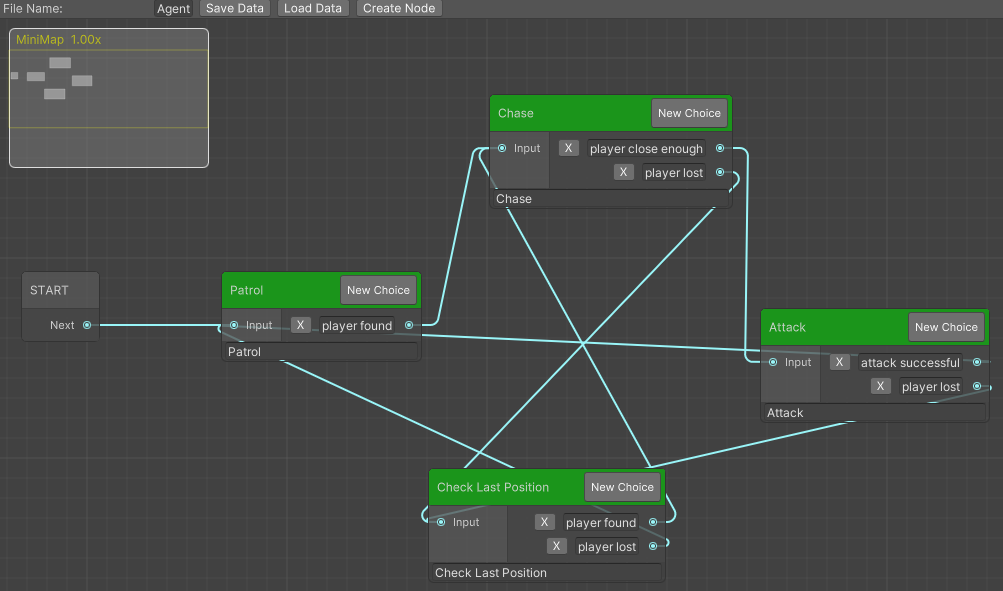
\includegraphics[scale=0.45]{images/sequence_graph_agent.png}
	\caption{Sequence graph example for an agent}
	\label{fig:sequence_graph_agent}
\end{figure}

This screenshot shows the behaviour of an agent patrolling the area around him. If it finds a player, it will try to attack them, and if it loses the player, it will check their last seen position. This is a fairly simple behaviour with only four states and eight edges, but it already looks very messy and hard to follow, and this problem will only get worse as it grows in size and complexity.

Another problem is loops and repeating sequences in general. As you can see in figure \ref{fig:sequence_graph_agent}, there are several loops built in, one of which is "Patrol" - "Chase" - "Check Last Position". There is no way to get rid of the loops in this example, and they are usually the cause of the disarray. As the name suggests, sequence graphs are excellent for sequential behaviour, like a dialogue graph or a shader graph, but struggle with an organised look when it comes to repeating behaviour.

Since the behaviour of a tour guide is sequential, a sequence graph would work well for it. However, this asset should become a tool that is useful for other types of behaviour as well, and many Non-Player Characters NPCs in games are based on repetitive behaviour. Therefore, a solution is needed that also supports loops, while retaining the flexibility of a graph.

In addition, as the complexity of a behaviour increases, it would be helpful if certain parts of the graph could be collapsed so that only the core parts remain visible. Unfortunately, this isn't possible in a graph that can contain loops, because any state can be connected to anywhere, and there is no tree-like structure that would allow this.

The FSMs could be organised into a hierarchical structure, by completely extracting certain parts of the graph, to make them easier to read. But this would still not solve the problem that they would become unmanageable once they reach a certain complexity.

All these problems combined together explain why this approach isn't optimal, however, a behaviour tree looks like it solves all of these issues.